\section{Self-Training Neural Operator} \label{sec:stno}

\subsection{Definition}
\noindent We propose to generalize the Neural Operator $\mathcal{G}_{\theta}^{T}$ so that it maps any point of the trajectory $\mathbf{x}_{t_n}$ to the trajectory between $[\mathbf{x}_{t_n}, \mathbf{x}_{\epsilon}]$:
\begin{align}
\mathcal{G}_{\theta} : (\mathbb{R}^d, \mathcal{T}) & \mapsto \mathbb{R}^{N \times d}\\
   \mathcal{G}_{\theta}(\mathbf{x}_{t_n}, t_n) &= Z_{N - n} \cup \left\{\widehat{\mathbf{x}}_{t_k}\right\}_{k \in [\epsilon, n ]} \: \: \forall \; t_{n} \in \mathcal{T} \setminus \epsilon \label{G:def}\\
   \mathcal{G}_{\theta}(\mathbf{x}_{\epsilon}, \epsilon) &= Z_{N - 1} \cup \mathbf{x}_{\epsilon}  \label{G:bound} \: \: \text{(Boundary Condition)} \\
\end{align}

\noindent Where $Z_{n} \in \mathbb{R}^{n \times d}$ is a matrix of zeros. Having $k \in [\epsilon, n ]$ ensures that the operator only computes the "forward" trajectory. The "backward" trajectory is set to 0 using $Z_{N - {n}}$. This ensures that the function has a fixed output space, which is useful both for analytical proofs and NN design. A visual summary of our operator is shown in Figure~\ref{fig:genno}\\

\begin{figure}[htbp]
  \centering
  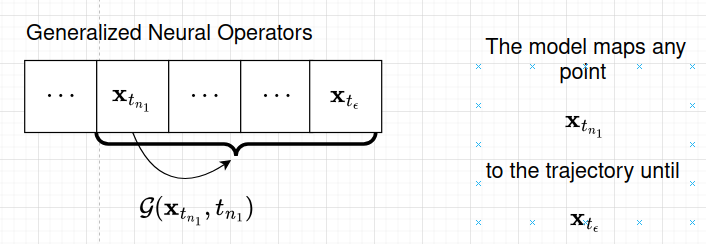
\includegraphics[width=0.5\textwidth]{figures/genno.png}
  \caption{A visual summary of our proposal approach.}
  \label{fig:genno}
\end{figure}

\subsection{Loss}

Suppose that we have a perfect trajectory estimator $\mathcal{G}(. \:, \:. \:; \phi)$, built upon an ODE solver $\Phi$ :
\begin{align}
    \mathcal{G}(\mathbf{x}_{t_n}, t_{n}; \phi) &= Z_{N - n - 1} \cup \left\{\widehat{\mathbf{x}}_{t_k}^{\phi}\right\}_{\forall k < n} \label{G:trainer}
\end{align}

\subsubsection{Distillation loss}
\noindent Drawing inspiration from \cite{song2023consistencymodels} Appendix~A.2 and A.3, we propose the following losses:
\begin{align}
    \mathcal{L}_{\Phi} \left(\theta, \theta^-; \phi \right) &= \mathbb{E}\left[ \lambda(t_n) d \left(\mathcal{G}_{\theta} (\mathbf{x}_{t_{n+1}}, t_{n+1}), \mathcal{G}_{\theta^-} (\widehat{\mathbf{x}}_{t_{n}}^{\phi}, t_{n}) \right)\right] \label{def:loss}
\end{align}

\noindent Where the metric function $d$ has the following properties:
\begin{align}
        d\left(\mathcal{G}_{\theta} (\mathbf{x}_{t_{n+1}}, t_{n+1}), \mathcal{G}_{\theta} (\mathbf{x}_{t_{n}}, t_{n})\right) &= d\left(\mathcal{G}_{\theta} (\mathbf{x}_{t_{n+1}}, t_{n+1})[1:n-1], \mathcal{G}_{\theta} (\mathbf{x}_{t_{n}}, t_{n})\right) \label{d:prop} \\
         d\left(\mathcal{G}_{\theta} (\mathbf{x}_{t_{n+1}}, t_{n+1}), \mathcal{G}_{\theta} (\mathbf{x}_{t_{n}}, t_{n})\right) & = 0 \\\Leftrightarrow \mathcal{G}_{\theta} (\mathbf{x}_{t_{n+1}}, t_{n+1})[1:n-1] & = \mathcal{G}_{\theta} (\mathbf{x}_{t_{n}}, t_{n})  \label{d:zero}
\end{align}
\noindent This adjustment ensures that the extra point $\widehat{\mathbf{x}}_{t_n}$, forecasted by $\mathcal{G}_{\theta} (\mathbf{x}_{t_{n+1}}, t_{n+1})$, is not compared to the zeros of $\mathcal{G}_{\theta} (\mathbf{x}_{t_{n}}, t_{n})$. The theoretical background for the choice of this loss can be found in the Appendix~\ref{app:ld}

\subsubsection{Self-Training Loss}

\noindent Based on the definition of the noising process:
\begin{align}
    \mathbf{x_{t_n}} = \mathbf{x} + t_nz \label{def:xtn}
\end{align}
\noindent where $z \sim \mathcal{N}(0, 1)$, we propose the following self-training loss, that does not depend on $\Phi$:
\begin{align}
    \mathcal{L}_{\Theta} \left(\theta, \theta^-\right) &= \mathbb{E}\left[ \lambda(t_n) d \left(\mathcal{G}_{\theta}(\mathbf{x} + t_{n+1}z, t_{n+1}), \mathcal{G}_{\theta^-}(\mathbf{x} + t_nz, t_{n}) \right)\right] \label{def:selfloss}
\end{align}

\noindent In the Appendix~\ref{app:loss}, we extend Theorem~2 of \cite{song2023consistencymodels} to support this proposition. 

\begin{comment}
    \section{Extension to Continuous Time}

We propose to extend our operator to continuous time to avoid discretization errors. 

\subsection{Loss}

Based on Theorem 6 of \cite{song2023consistencymodels}, we employ the following continuous loss:

\begin{align}
    \mathcal{L}_{\Omega}\left(\theta, \theta^- \right) = \mathbb{E} \left[ \frac{\lambda(t)}{(\tau^{-1})^{'}(t)}\mathcal{G}_{\theta}(\mathbf{x}_t, t)^T H(\mathcal{G}_{\theta^{-}}(\mathbf{x}_t, t)) \frac{d \mathcal{G}_{\theta^{-}}(\mathbf{x}_t, t)}{dt} \right]
\end{align}

\noindent Where $\tau(\frac{n - 1}{N -1}) = t_n$  and $[H(\mathbf{x})]_{i, j} = \frac{\delta^2d(y, x)}{\delta y_i \delta y_j} \lvert_{x=y}$. Additional details about the choice of this loss are given in the Appendix~\ref{app:continuous}. Note that this loss is only meaningful in terms of its gradient, not in terms of its value.

\subsection{TrigFlow Parametrization}

Following Section~3 of \cite{lu2025simplifyingstabilizingscalingcontinuoustime}, we rewrite our operator as : 

\begin{align}
    \mathcal{G}_{\theta}(\mathbf{x}_t, t) = cos(t) \mathbf{x}_t - sin(t) \sigma_d G_{\theta} \left(\frac{\mathbf{x}_t}{\sigma_d}, t \right)
\end{align}

\noindent Where $G_{\theta}$ is a Neural Network trained with parameters $\theta$, whose output is zero-padded using matrices $Z$. Note that they obtain these results empirically by remarking the stability over the terms of
\begin{align}
    \frac{d f_{\theta^{-}}(\mathbf{x}_t, t)}{dt} = -cos(t)\left(\sigma_d F_{\theta^{-}}\left(\frac{\mathbf{x}_t}{\sigma_d} \right) - \frac{d\mathbf{x}}{dt}\right) - sin(t) \left(\mathbf{x} + \sigma_d \left(\frac{d F_{\theta^{-}}\left(\frac{\mathbf{x}_t}{\sigma_d} \right)}{dt} \right) \right)
\end{align}
\noindent We give a justification for why these findings can apply to $\mathcal{G}$ in the Appendix~\ref{app:trigflow}

\subsection{Adaptive Weighting}

We also reformulate the loss using the adaptive weighting function $\omega_{\psi}(t)$ from Section~4 of \cite{lu2025simplifyingstabilizingscalingcontinuoustime}, that is learned from data using parameters $\psi$
\begin{align}
    \mathcal{L}_{\Psi}(\theta, \theta^{-}) & = \mathbb{E} \left[ \frac{e^{\omega_{\psi}(t)}}{d} \left\lVert G_{\theta}\left( \frac{\mathbf{x_t}}{\sigma_d}, t \right) - G_{\theta^{-}}\left( \frac{\mathbf{x_t}}{\sigma_d}, t \right) - cos(t) \frac{d \mathcal{G}_{\theta^{-}}(\mathbf{x_t}, t)}{dt}\right\rVert_2^2  - \omega_{\psi}(t) \right]
\end{align}

\noindent This finding is based on the fact that $\nabla\mathbb{E}\left[F_{\theta}^Ty\right] = \frac{1}{2} \nabla\mathbb{E}\left[ \left\lVert F_{\theta} - F_{\theta^{-}} - y \right\rVert_2^2\right]$ (see Appendix~D of \cite{lu2025simplifyingstabilizingscalingcontinuoustime}. The given proof is agnostic of which function $F_{\theta}$ is employed so we directly extend it to $\mathcal{G}$

\subsection{JVP re-arrangement}

Lastly, we also rewrite the computation of the tangent, using findings from Section~5 of \cite{lu2025simplifyingstabilizingscalingcontinuoustime}:

\begin{align}
 cos(t)\frac{d \mathcal{G}_{\theta^{-}}(\mathbf{x_t}, t)}{dt} & \sim cos(t)sin(t) \frac{d G_{\theta^{-}}(\mathbf{x_t}, t)}{dt} \\
 g & = cos(t)sin(t) \left( \nabla_{\mathbf{x_t}\sigma_d^{-1}} G_{\theta^{-}}(\mathbf{x_t}, t)\right)\frac{d x_t}{dt} + \delta t G_{\theta^{-}}(\mathbf{x_t}, t) \sigma_d \\
 g & = JVP\left(G_{\theta^{-}}(\mathbf{x_t}\sigma_d^{-1}, t), (cos(t)sin(t)\frac{d x_t}{dt}, \frac{d x_t}{dt}\sigma_d)\right)
\end{align}

\noindent Here, it's only a matter of re-writing the tangent computation to improve numerical stability. Hence, this results applies to $\mathcal{G}$

\noindent We also apply tangent normalization to this expression: $g = \frac{g}{\lVert g \rVert + c}$.

\end{comment}